\documentclass[ignorenonframetext,hyperref={pdftex,unicode},compress,handout]{beamer}
\mode<presentation>{}
\usepackage[utf8]{inputenc}
\usepackage[russian]{babel}
\usepackage[T2A]{fontenc}
\usepackage{amssymb,amsfonts,amsmath,mathtext}


\usetheme{Pittsburgh}
% for handout only
\usecolortheme{dove}


\newcommand{\br}{\vspace{12pt}}
\newtheorem{teo}{Теорема}
\newtheorem{alg}{Алгоритм}


%-------------------------------------------------------------------------------


\title{Параметризация управлений в системах с марковскими переключениями и задачах робастной стабилизации.}
\author{Архипов С.\,В.}
\institute{Научный руководитель: Пакшин П.\,В.}
\date{16 июня 2009 г.}



\begin{document}



%-------------------------------------------------------------------------------
%---   слайд 0: титульная страница
%-------------------------------------------------------------------------------
\begin{frame}
\titlepage
\end{frame}



%-------------------------------------------------------------------------------
%---   слайд 1: постановка основной задачи
%-------------------------------------------------------------------------------
\begin{frame}
    \frametitle{Проблема синтеза управления}
    \framesubtitle{Постановка основной задачи}
    \begin{equation} % (1)
        \left\{
            \begin{array}{l}
                \dot{x} = Ax + Bu\mbox{,} \\
                y = Cx\mbox{,} \\
                u = -F_0y\mbox{.}
            \end{array}
        \right.
    \end{equation}
    \br
    \begin{description}
        \item[x(t)]~--- вектор состояний динамической системы,
        \item[y(t)]~--- вектор выходов,
        \item[u(t)]~--- вектор управлений.
    \end{description}
    \br
    \par Необходимо построить такое $u(t)$, которое бы \alert{наилучшим образом} соответствовало некоторому критерию.
\end{frame}




%-------------------------------------------------------------------------------
%---   слайд 2: синтез управления
%-------------------------------------------------------------------------------
\begin{frame}
    \frametitle{Проблема синтеза управления}
    \framesubtitle{Синтез управления}
    \par Если $P>0$ и $F$ подходящих размерностей, то система стабилизируема тогда и только тогда, когда
    \begin{equation} % (2)
        P(A-BF)+(A-BF)^TP < 0\mbox{.}
    \end{equation}
    \br
    \par После замены $W=P^{-1}$ матрица $F=F_0C$ может быть найдена из неравенства
    \begin{equation}
        (A-BF_0C)W+W(A-BF_0C)^T < 0\mbox{.}
    \end{equation}
\end{frame}




%-------------------------------------------------------------------------------
%---   слайд 3: $W$-проблема
%-------------------------------------------------------------------------------
\begin{frame}
    \frametitle{Проблема синтеза управления}
    \framesubtitle{Метод Крузиуса--Трофино}
    \par Необходимо найти матрицы $W$, $N$ и $M$ такие, что
    \begin{equation}
        \left\{
            \begin{array}{l}
                AW + WA^T - BNC - C^TN^TB^T < 0\mbox{,} \\
                W > 0\mbox{,} \\
                MC = CW\mbox{.}
            \end{array}
        \right.
    \end{equation}
    \br
    Тогда
    \begin{equation}
        u = -NM^{-1} = -F_0y\mbox{.}
    \end{equation}
\end{frame}




%-------------------------------------------------------------------------------
%---   слайд 4: формализация основной задачи
%-------------------------------------------------------------------------------
\begin{frame}
    \frametitle{Параметризация управлений}
    \framesubtitle{Формализация задачи}
    \begin{equation}
        \left\{
            \begin{array}{l}
                \dot{x}(t) = A\big( r(t) \big) + B\big( r(t) \big) u(t)\mbox{,} \\
                y(t) = C\big( r(t) \big)\mbox{,} \\
                u(t) = -F_iy\mbox{ при } r(t)=i\mbox{.}
            \end{array}
        \right.
    \end{equation}
    \br
    \begin{description}
        \item[r(t)]~--- процесс переключений, моделируемый однородной марковской цепью с вероятностями переходов
    \end{description}
    \begin{equation}
        \mathbf{P}\big(r(t+h) = j~|~r(t) = i \big) = \left\{
            \begin{array}{ll}
                \pi_{ij} + o(h) & \mbox{ при } i \neq j\mbox{,} \\
                1 + \pi_{ij} + o(h) & \mbox{ при } i = j\mbox{.} \\
            \end{array}
        \right.
    \end{equation}
\end{frame}




%-------------------------------------------------------------------------------
%---   слайд 5: теорема о существовании матриц усиления
%-------------------------------------------------------------------------------
\begin{frame}
    \frametitle{Параметризация управлений}
    \framesubtitle{Теорема о существовании матриц усиления}
    \small
    \begin{teo}
        \par Матрицы усиления $F_i$ существует тогда и только тогда, когда найдутся такие матрицы параметров $Q_i = Q_i^T \geqslant 0$ и $R_i = R_i^T \geqslant 0$, что
        \begin{equation}
            F_iC = R_i^{-1}\big[ B_i^TH_i + L_i \big]\mbox{.}
        \end{equation}
        \br
        \par $H_i = H_i^T > 0$ и $L_i$ находятся из
        \begin{equation}
            \left\{
                \begin{array}{l}
                    A_i^T + H_iA_i - H_iB_iR_i^{-1}B_i^TH_i + Q_i + \\
                    + \sum_{j=1}^N \pi_{ij}H_j + L_i^TR_i^{-1}L_i < 0\mbox{.}
                \end{array}
            \right.
        \end{equation}
    \end{teo}
\end{frame}




%-------------------------------------------------------------------------------
%---   слайд 6: задача робастной стабилизации
%-------------------------------------------------------------------------------
\begin{frame}
    \frametitle{Параметризация управлений}
    \framesubtitle{Задача робастной стабилизации}
    \begin{equation}
        \left\{
            \begin{array}{l}
                \dot{x}(t) = \sum\limits_{i=1}^N \xi i(t)\big[ A_ix(t) + B_iu(t) \big]\mbox{,} \\
                y(t) = Cx(t)\mbox{,} \\
                u(t) = -Fy(t)\mbox{.}
            \end{array}
        \right.
    \end{equation}
    \br
    \begin{equation}
        \left\{
            \begin{array}{l}
                \xi_i(t) \geqslant 0\mbox{,} \\
                \sum_{i=1}^N\xi_i(t) = 1\mbox{.}
            \end{array}
        \right.
    \end{equation}
\end{frame}




%-------------------------------------------------------------------------------
%---   слайд 7: задача робастной стабилизации (слайд 2)
%-------------------------------------------------------------------------------
\begin{frame}
    \frametitle{Параметризация управлений}
    \framesubtitle{Задача робастной стабилизации}
    \begin{teo}
        \par Матрица усиления $F$ будет обеспечивать требуемую устойчивость тогда и только тогда, когда найдутся матрицы параметров $Q_i = Q_i^T \geqslant 0$ и $R_i = R_i^T > 0$, что выполняется уравнение
        \begin{equation}
            FC = R_i^{-1}\big[ B_i^TH + L_i \big]\mbox{.}
        \end{equation}
        \br
        \par $L_i$ и $H_i = H = H^T > 0$~--- решения системы матричных уравнений
        \begin{equation}
            A_i^TH + HA - HB_iR_i^{-1}B_i^TH + Q_i + L_i^TR_i^{-1}L_i < 0
        \end{equation}
        \par для всех $i \in \mathcal{N}$.
    \end{teo}
\end{frame}





%-------------------------------------------------------------------------------
%---   слайд 8: алгоритм решения задачи робастной стабилизации
%-------------------------------------------------------------------------------
\begin{frame}
    \frametitle{Параметризация управлений}
    \framesubtitle{Алгоритм решения задачи робастной стабилизации}
    \small
    \begin{alg}
        \begin{enumerate}
            \item
            \par Решим матричные неравенства и уравнения относительно $X_i$, $Y_i$, $M_i$ и $K$:
            \begin{equation}
            \label{eq:1}
                \left\{
                    \begin{array}{l}
                        \left(
                            \begin{array}{ccc}
                                XA_i^T + A_iX - B_iR_i^{-1}B_i   &   X_i\sqrt{Q_i}   &   Y_i^T   \\
                                \sqrt{Q_i}X   &   -E   &   0 \\
                                Y_i   &   0   &   -R_i
                            \end{array}
                        \right) < 0\mbox{,} \\
                        CX = M_iC\mbox{,} \\
                        K = R_i^{-1}(B_i^T + Y_i)\mbox{,} \\
                        (B_i^T + Y_i)(R - C^+C) = 0\mbox{.}
                    \end{array}
                \right.
            \end{equation}

            \item
            \par Если \ref{eq:1} разрешима, то
            \begin{equation}
                F = \big[ R_i^{-1}(B_i^T + Y_i)C^+ + Z(E + C^+C) \big]M_i^{-1}\mbox{.}
            \end{equation}
        \end{enumerate}
    \end{alg}
\end{frame}





%-------------------------------------------------------------------------------
%---   слайд 9: задача одновременной стабилизации
%-------------------------------------------------------------------------------
%\begin{frame}
%    \frametitle{Параметризация управлений}
%    \framesubtitle{Задача одновременной стабилизации}
%    \begin{equation}
%        \left\{
%            \begin{array}{l}
%                \dot{x}(t) = A_ix(t) + B_iu(t)\mbox{,} \\
%                y(t) = Cx(t)\mbox{,} \\
%                u(t) = -Fy(t)\mbox{.}
%            \end{array}
%        \right.
%    \end{equation}
%\end{frame}




%-------------------------------------------------------------------------------
%---   слайд 10: задача одновременной стабилизации (слайд 2)
%-------------------------------------------------------------------------------
%\begin{frame}
%    \frametitle{Параметризация управлений}
%    \framesubtitle{Задача одновременной стабилизации}
%    \begin{teo}
%        \par Матрица усиления $F$ будет обеспечивать требуемую устойчивость тогда и только тогда, когда найдутся матрицы параметров $Q_i = Q_i^T \geqslant 0$ и $R_i = R_i^T > 0$, что выполняется уравнение
%        \begin{equation}
%            FC = R_i^{-1}\big[ B_i^TH_i + L_i \big]\mbox{.}
%        \end{equation}
%        \br
%        \par $L_i$ и $H_i = H_i^T > 0$~--- решения системы матричных уравнений
%        \begin{equation}
%            A_i^TH_i + H_iA - H_iB_iR_i^{-1}B_i^TH_i + Q_i + L_i^TR_i^{-1}L_i < 0
%        \end{equation}
%        \par для всех $i \in \mathcal{N}$.
%    \end{teo}
%\end{frame}






%-------------------------------------------------------------------------------
%---   слайд 11: алгоритм решения задачи одновременной стабилизации
%-------------------------------------------------------------------------------
%\begin{frame}
%    \frametitle{Параметризация управлений}
%    \framesubtitle{Алгоритм решения задачи одновременной стабилизации}
%    \small
%    \begin{alg}
%        \begin{enumerate}
%            \item
%            \par Решим матричные неравенства и уравнения относительно $X_i$, $Y_i$, $M_i$ и $K$:
%            \begin{equation}
%            \label{eq:2}
%                \left\{
%                    \begin{array}{l}
%                        \left(
%                            \begin{array}{ccc}
%                                X_iA_i^T + A_iX_i - B_iR_i^{-1}B_i   &   X_i\sqrt{Q_i}   &   Y_i^T   \\
%                                \sqrt{Q_i}X_i   &   -E   &   0 \\
%                                Y_i   &   0   &   -R_i
%                            \end{array}
%                        \right) < 0\mbox{,} \\
%                        C_iX_i = M_iC_i\mbox{,} \\
%                        K = R_i^{-1}(B_i^T + Y_i)\mbox{,} \\
%                        (B_i^T + Y_i)(R - C_i^+C_i) = 0\mbox{.}
%                    \end{array}
%                \right.
%            \end{equation}

%            \item
%            \par Если \ref{eq:2} разрешима, то
%            \begin{equation}
%                F = \big[ R_i^{-1}(B_i^T + Y_i)C^+ + Z(E + C^+C) \big]M_i^{-1}\mbox{.}
%            \end{equation}
%        \end{enumerate}
%    \end{alg}
%\end{frame}






%-------------------------------------------------------------------------------
%---   слайд 12: задача пассификации
%-------------------------------------------------------------------------------
\begin{frame}
    \frametitle{Параметризация управлений}
    \framesubtitle{Задача пассификации}
    \begin{equation}
        \left\{
            \begin{array}{l}
                \dot{x}(t) = Ax(t) + Bu(t) + \sum\limits_{i=1}^N \delta_i(t)\big[ A_ix(t) + B_iu(t) \big]\mbox{,} \\
                y(t) = Cx(t)\mbox{,} \\
                u = \omega - Fy\mbox{,} \\
                z = Gy\mbox{.}
            \end{array}
        \right.
    \end{equation}
    \begin{eqnarray}
        \underline{\delta}_i \leqslant \delta_i(t) \leqslant \overline{\delta}_i\mbox{,} \\
        \Delta_0 = \big\{ \delta(t)~|~ \delta_i \in \{ \underline{\delta}_i, \overline{\delta}_i \} \big\}\mbox{,}
    \end{eqnarray}
\end{frame}




%-------------------------------------------------------------------------------
%---   слайд 13: задача пассификации (слайд 2)
%-------------------------------------------------------------------------------
\begin{frame}
    \frametitle{Параметризация управлений}
    \framesubtitle{Задача пассификации}
    \par Условие \alert{строгой $G$-пассивности}
    \begin{equation}
        V(x) \leqslant V(x_0) + \int\limits_0^t \big( u^T(s)Gy(s) - \mu(x(s)) \big)\,ds
    \end{equation}
    \par можно переписать в виде
    \begin{equation}
        \left(
            \begin{array}{cc}
                A_c^T(\delta)H + HA_c(\delta) + M   &   HB(\delta) - (GC)^T \\
                B^T(\delta)H - GC   &   0
            \end{array}
        \right) \leqslant 0\mbox{,}
    \end{equation}
    \par где $A_c(\delta) = A(\delta) - B(\delta)FC$.
\end{frame}






%-------------------------------------------------------------------------------
%---   слайд 14: задача пассификации (слайд 3)
%-------------------------------------------------------------------------------
\begin{frame}
    \frametitle{Параметризация управлений}
    \framesubtitle{Задача пассификации}
    \small
    \begin{teo}
        \par Матрица усиления $F$, обеспечивающая требуемую устойчивость, будет существовать тогда и только тогда, когда найдутся матрицы параметров $Q = Q^T \geqslant 0$ и $R = R^T > 0$, что
        \begin{equation}
            FC = R^{-1}\big[ B^T(\delta)P + L(\delta) \big] \mbox{ при всех } \delta \in \Delta_0{,}
        \end{equation}
        \par где $P = P^T > 0$ и $L(\delta)$ есть решения матричного неравенства
        \begin{equation}
            A^T(\delta)P + PA(\delta) - PB(\delta)R^{-1}B^T(\delta)P + Q + L^T(\delta)R^{-1}L(\delta) < 0\mbox{.}
        \end{equation}
    \end{teo}
\end{frame}





%-------------------------------------------------------------------------------
%---   слайд 15: задача пассификации (слайд 3)
%-------------------------------------------------------------------------------
\begin{frame}
    \frametitle{Параметризация управлений}
    \framesubtitle{Синтез пассифицирующей обратной связи}
    \tiny
    \begin{alg}
        \begin{enumerate}
            \item
            \par Решим матричные неравенства и уравнения относительно $X$, $Y(\delta)$, $M$ и $K$:
            \begin{equation}
            \label{eq:3}
                \left\{
                    \begin{array}{l}
                        \left(
                            \begin{array}{ccc}
                                XA^T(\delta) + A(\delta)X - B^T(\delta)R^{-1}B(\delta)   &   X\sqrt{Q}   &   Y^T(\delta)   \\
                                \sqrt{Q}X   &   -E   &   0 \\
                                Y(\delta)   &   0   &   -E
                            \end{array}
                        \right) < 0\mbox{,} \\
                        CX = MC\mbox{,} \\
                        K = R_i^{-1}(B^T(\delta) + Y(\delta))\mbox{,} \\
                        (B^T(\delta) + Y(\delta))(E - C^+C) = 0\mbox{.}
                    \end{array}
                \right.
            \end{equation}

            \item
            \par Если \ref{eq:3} разрешима, то
            \begin{equation}
                F = \big[ R^{-1}(B^T(\delta) + Y(\delta))C^+ + Z(E + C^+C) \big]M^{-1}\mbox{.}
            \end{equation}

            \item
            \par Если \ref{eq:3} разрешима, то решим следующее неравенство относительно $G$ и $H = H^T > 0$:
            \begin{equation}
                \left(
                    \begin{array}{cc}
                        A^T_c(\delta)H + HA_c(\delta) + W   &   HB(\delta) + (GC)^T \\
                        B^T(\delta)H - GC   &   0
                    \end{array}
                \right) \leqslant 0\mbox{,}
            \end{equation}
            \par откуда найдем $G$.
        \end{enumerate}
    \end{alg}
\end{frame}





%-------------------------------------------------------------------------------
%---   слайд 16: пример
%-------------------------------------------------------------------------------
\begin{frame}
    \frametitle{Пример}
    \framesubtitle{Автоматическое управление полетом самолета}
        \begin{equation}
            \left\{
                \begin{array}{l}
                    \dot{\vartheta} = \omega_z\mbox{,} \\
                    \dot{\omega}_z = -a_{mz}^\alpha\vartheta - a_{mz}^{\omega z}\omega_z + a_{mz}^\alpha\Theta + a_{mz}^\delta\delta\mbox{,} \\
                    \dot{\Theta} = -a_y^\alpha\vartheta + a_y^\alpha\Theta\mbox{,} \\
                    u(t) = \delta\mbox{.}
                \end{array}
            \right.
        \end{equation}
        \br
        \begin{description}
            \item[$\vartheta$]~--- угол тангажа,
            \item[$\omega_z$]~--- угловая скорость тангажа,
            \item[$\Theta$]~--- угол наклона траектории,
            \item[$\alpha$]~--- угол атаки,
            \item[$\delta$]~--- угол отклонения руля.
        \end{description}
\end{frame}





%-------------------------------------------------------------------------------
%---   слайд 17: пример (слайд 2)
%-------------------------------------------------------------------------------
\begin{frame}
    \frametitle{Пример}
    \framesubtitle{Автоматическое управление полетом самолета}
        \begin{equation*}
            \begin{array}{cc}
                A_1^0 = \left(
                    \begin{array}{ccc}
                        0     &     1     &     0 \\
                        -14.19    &     -6.08   &     14.19 \\
                        -2.96  &     0     &     -2.96
                    \end{array}
                \right)\mbox{,} &
                B_1^0 = \left(
                    \begin{array}{c}
                        0 \\
                        -7.64 \\
                        0
                    \end{array}
                \right)\mbox{;} \\
                \vdots   &   \vdots \\
                A_9^0 = \left(
                    \begin{array}{ccc}
                        0     &     1     &     0 \\
                        -110.56    &     -6.05   &     110.56 \\
                        0.61  &     0     &     -0.61
                    \end{array}
                \right)\mbox{,} &
                B_9^0 = \left(
                    \begin{array}{c}
                        0 \\
                        -53.49 \\
                        0
                    \end{array}
                \right)\mbox{;} \\ \\
                C_{i0} = \left(
                    \begin{array}{ccc}
                        1 & 0 & 0 \\
                        0 & 1 & 0
                    \end{array}
                \right)\mbox{,} &
                i \in \{1,2,\ldots,N\}\mbox{.}
            \end{array}
        \end{equation*}
\end{frame}




%-------------------------------------------------------------------------------
%---   слайд 18: пример (слайд 3)
%-------------------------------------------------------------------------------
\begin{frame}
    \frametitle{Пример}
    \framesubtitle{Автоматическое управление полетом самолета}
    \begin{eqnarray*}
        F^1&=&\left[~-9.01~~-1~\right] \\
        F^2&=&\left[~-11.4~~-0.9~\right]
    \end{eqnarray*}
\end{frame}





%-------------------------------------------------------------------------------
%---   слайд 19: пример (слайд 4)
%-------------------------------------------------------------------------------
\begin{frame}
    \frametitle{Пример}
    \framesubtitle{Автоматическое управление полетом самолета}
    \br
    \begin{center}
    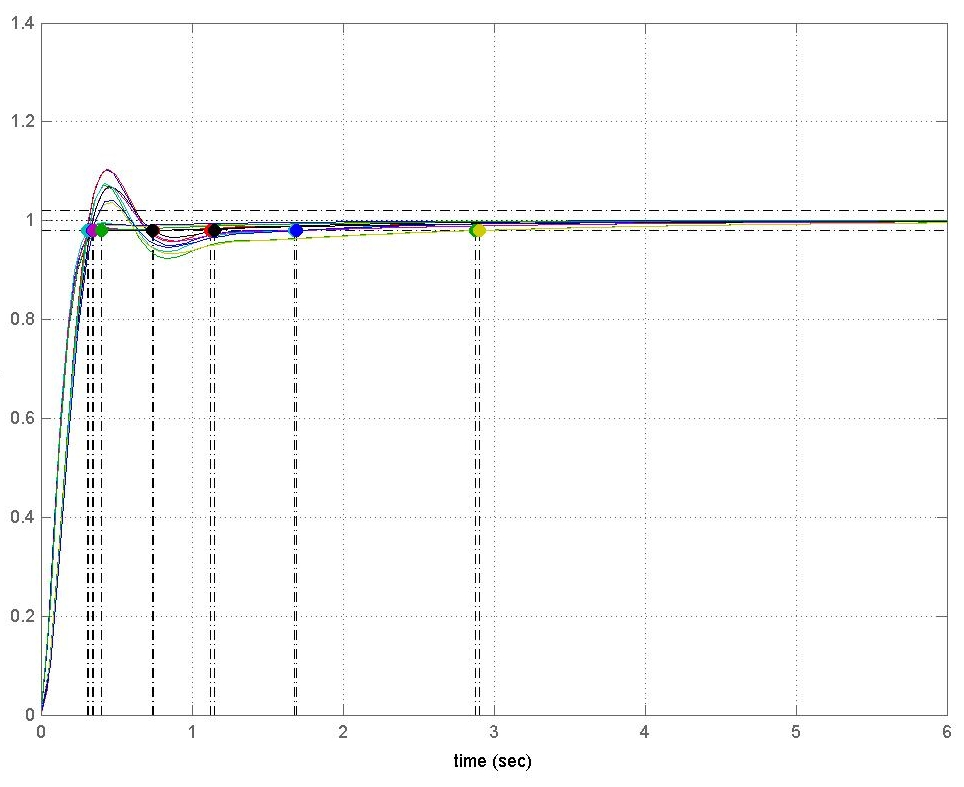
\includegraphics[height=7cm]{shot.jpg}
    \end{center}
\end{frame}






%-------------------------------------------------------------------------------
%---   слайд 20: пример (слайд 2)
%-------------------------------------------------------------------------------
\begin{frame}
    \frametitle{Пример}
    \framesubtitle{Автоматическое управление полетом самолета}
        \begin{equation*}
            \begin{array}{cc}
                A_1^0 = \left(
                    \begin{array}{ccc}
                        0     &     1     &     0 \\
                        -6    &     1   &     6 \\
                        0  &     0     &     0
                    \end{array}
                \right)\mbox{,} &
                B_1^0 = \left(
                    \begin{array}{c}
                        0 \\
                        -4 \\
                        0
                    \end{array}
                \right)\mbox{;} \\
                \vdots   &   \vdots \\
                A_9^0 = \left(
                    \begin{array}{ccc}
                        0     &     1     &     0 \\
                        -25    &     0   &     28 \\
                        20  &     0     &     -20
                    \end{array}
                \right)\mbox{,} &
                B_9^0 = \left(
                    \begin{array}{c}
                        0 \\
                        0 \\
                        0
                    \end{array}
                \right)\mbox{;} \\ \\
                C_{i0} = \left(
                    \begin{array}{ccc}
                        1 & 0 & 0 \\
                        0 & 1 & 0
                    \end{array}
                \right)\mbox{,} &
                i \in \{1,2,\ldots,N\}\mbox{.}
            \end{array}
        \end{equation*}
\end{frame}







%-------------------------------------------------------------------------------
%---   слайд 21: заключение
%-------------------------------------------------------------------------------
\begin{frame}
    \frametitle{Заключение}
    \begin{itemize}
        \item Исследована исходная задача управления;
        \item Приведен метод Крузиуса--Трофино решения невыпуклой задачи;
        \item Полученные результаты распространены на случай стохастических систем;
        \item Предложены алгоритмы решения некоторых прикладных задач теории управления;
        \item Даны условия реализуемости алгоритмов.
    \end{itemize}
\end{frame}




\end{document}
